\chapter{Einleitung}

Mit der steigenden Menge von benutzergenerierten Inhalten steigt auch die Menge von Metadaten, die mit diesen Inhalten verknüpft sind. Zur späteren Durchsuchbarkeit und Kategorisierung geben viele Online-Plattformen, Marktplätze und Online-Shops ihren Benutzern die Möglichkeit, Inhalte mit Metadaten zu versehen.

Eine oft genutzte Möglichkeit zur Beschreibung von Inhalten sind Tags. Dabei handelt es sich um Wörter oder Wortgruppen, die vom Benutzer frei gewählt werden können, um den Inhalt zu beschreiben. Dabei unterliegt die Eingabe von Tags möglichst wenigen Regeln, um dem Benutzer eine für ihn natürliche Beschreibung des Inhaltes zu ermöglichen. Dabei ist explizit, im Gegensatz zu einer Kategorisierung, die Vergabe von mehreren Tags vorgesehen \cite{sc2005}.

Ein charakteristisches Merkmal von Tags ist dabei, dass sie nur einen bestimmten Aspekt des getaggten Objektes beschreiben. Dabei sind Tags nicht hierarchisch und es werden an keiner Stelle vom Nutzer explizite Zusammenhänge zwischen Tags erstellt. Jedoch liegt die Annahme, dass zwischen Tags Beziehungen herstellbar sind und sich mehrere Tags zu übergeordneten Themen zusammenfassen lassen, nahe. Der Benutzer berücksichtigt diese Beziehungen bei der Eingabe des Tags, formuliert sie jedoch nicht explizit. Die nachträgliche Rekonstruktion der Denkprozesse bei der Eingabe von Tags ist Thema dieser Arbeit.

Dabei ist zu beachten, dass Benutzer bei der Eingabe von Tags unterschiedliche Ziele verfolgen. Idealerweise werden Tags so vergeben, dass sie das getaggte Objekt inhaltlich beschreiben. Jedoch werden vom Benutzer bei der Eingabe des Tags weitere Assoziationen hergestellt. Beispielsweise kann der Benutzer mit einem Objekt bestimmte Emotionen oder Wertungen verbinden, die sich in den vergebenen Tags widerspiegeln.

Auf Marktplätzen, bei denen Verkäufern die Möglichkeit des Taggings ihre Produkte gegeben wird, besteht eine weitere Motivation in der Erhöhung der Auffindbarkeit des Produktes. Dabei kann die inhaltliche Qualität des Tags außer Acht gelassen werden, wenn bei Vergabe einer falschen Beschreibung die Sichtbarkeit des Produktes erhöht wird. Auch der Marktplatzbetreiber selbst kann so vorgehen, um zu versuchen, die Gesamtverkäufe zu steigern.

Die verschiedenen Motivationen der Benutzern von Tags erschweren die nachträgliche Suche nach Assoziationen. Die vorliegende Masterarbeit beschäftigt sich mit Strategien zur Datenaufbereitung und Nutzung externer und interner Datenquellen und deren Integration mit Tag-Daten. Aus diesen Datenquellen wird eine Datenstruktur mit einem Kookkurenzgraphen als Basis aufgebaut. Außerdem wird eine Optimierung der verwendeten Parameter, die Evalutaion der Ergebnisse und eine Analyse der verwendeten Methoden durchgeführt.

\section{Motivation und Anwendungen}

Die nachträgliche Herstellung von Assoziationen in vorhandenen Tag-Daten bietet einige Nutzungsmöglichkeiten für den Betreiber der Online-Plattform.

Die Beziehungen zwischen Tags können genutzt werden, um Suchergebnisse zu verbessern. Wenn zu einem Suchbegiff weitere relevante Begriffe bekannt sind, können diese im Suchergebnis mit enthalten sein um somit auch Objekte zu finden, die nicht direkt mit dem Suchbegriff getaggt sind. Außerdem können Suchen vom Benutzer mit Hilfe von verwandten Tags verfeinert werden.

Über die Zusammenfassung von Tags zu Themen lässt sich außerdem die Navigation einer Website verbessern. Aus den Themen lassen sich Kategorien oder Hierarchien von Kategorien erzeugen, die besser den Denkmustern von Benutzern entsprechen. So sind auch Navigationskonzepte denkbar, die nicht hierarchisch, sondern assoziativ aufgebaut sind. Des weiteren können Tag-Assoziationen für Empfehlungssysteme genutzt werden, die einem Kunden zu einem bestimmten Artikel passende andere Artikel vorschlagen.

Im Bereich des Marketings können Beziehungen zwischen Tags genutzt werden, um für bestimmte externe Suchbegriffe spezielle Seiten zu erstellen (Landing Pages), die Inhalte zu diesem Suchbegriff bereitstellen oder Werbung für diese Suchbegriffe zu schalten. Außerdem können mit Hilfe des Kaufinteresses an bestimmten Themen über die Zeit Trends erkannt werden und mit entsprechenden Marketingmaßnahmen darauf reagiert werden.

All diese Anwendungen führen zu einer besseren Erfahrung für den Benutzer der Plattform. Die Präsentation von Daten kann besser auf die Denkmuster und Erwartungshaltungen des Benutzers angepasst werden. Dies führt in Konsequenz zu einem wirtschaftlichen Vorteil für den Plattformbetreiber.

\section{Kontext}   
\label{spreadshirt}

Die vorliegende Masterarbeit wurde im Kontext der sprd.net AG (Spreadshirt) \footnote{\url{http://www.spreadshirt.net}} erstellt. Spreadshirt ist eine E-Commerce-Plattform, die es seinen Benutzern erlaubt, personalisierte Textilien und andere Artikel zu gestalten, zu kaufen und zum Verkauf anzubieten. Spreadshirt übernimmt die Produktion und den Versand der Produkte. Ein Produkt bezeichnet hierbei einen Produkttyp, beispielsweise ein T-Shirt, das mit einem oder mehreren Designs bedruckt wurde.

Das Erstellen von Designs und die Konfiguration eines Produktes, also das Positionieren von Designs auf Produkttypen, wird dabei vollständig vom Benutzer durchgeführt. Spreadshirt bietet hierzu sowohl eine Website als auch eine API an.

Dabei agieren grundsätzlich zwei Arten von Benutzern mit der Spreadshirt-Plattform: \emph{Kunden} und \emph{Partner}.

Als Kunden werden Benutzer bezeichnet, die Produkte bestellen. Diese Produkte können entweder von ihnen selbst oder von einem Partner erstellt worden sein. 

Partner sind Benutzer, die Designs oder Produkte erstellen und diese zum Verkauf anbieten. Zu diesem Zweck kann der Partner einen eigenen Shop auf der Spreadshirt-Plattform eröffnen. Kunden können in diesem Shop Produkte bestellen und der Partner erhält einen Anteil des Verkaufspreises, während Spreadshirt die Produktion und den Versand an den Kunden übernimmt.

\begin{figure}
\label{fig:logo}
\begin{center}
    
\includegraphics[width=0.2\textwidth]{sprd_logo}
\end{center}
\caption{Spreadshirt-Logo}
\end{figure}

Neben den von Kunden für sich selbst erstellten Produkten und den Partner-Shops existiert ein weiterer Vertriebskanal: der Spreadshirt-Marktplatz. Auf dem Marktplatz können Partner nach ihrer Zustimmung ihre Designs vertreiben. Kunden können nach Motiven suchen, die ihrem Geschmack entsprechen und diese bestellen, mit anderen Motiven kombinieren oder mit Texten versehen.

Das Suchergebnis für Suchen auf dem Marktplatz hängt dabei maßgeblich von den Metadaten ab, die der Partner für seine Designs vergeben hat. Dies birgt auch Risiken: zur besseren Auffindbarkeit ihrer Designs sind Partner dadurch geneigt, populäre Tags zu vergeben, damit sie im Suchergebnis höher gewertet werden. Dies führt zu \emph{Spam} - Tags, die nicht erwünscht sind und den Inhalt des Designs nicht oder falsch beschreiben.

\begin{figure}[h]
\label{fig:howspreadshirtworks}
\begin{center}
    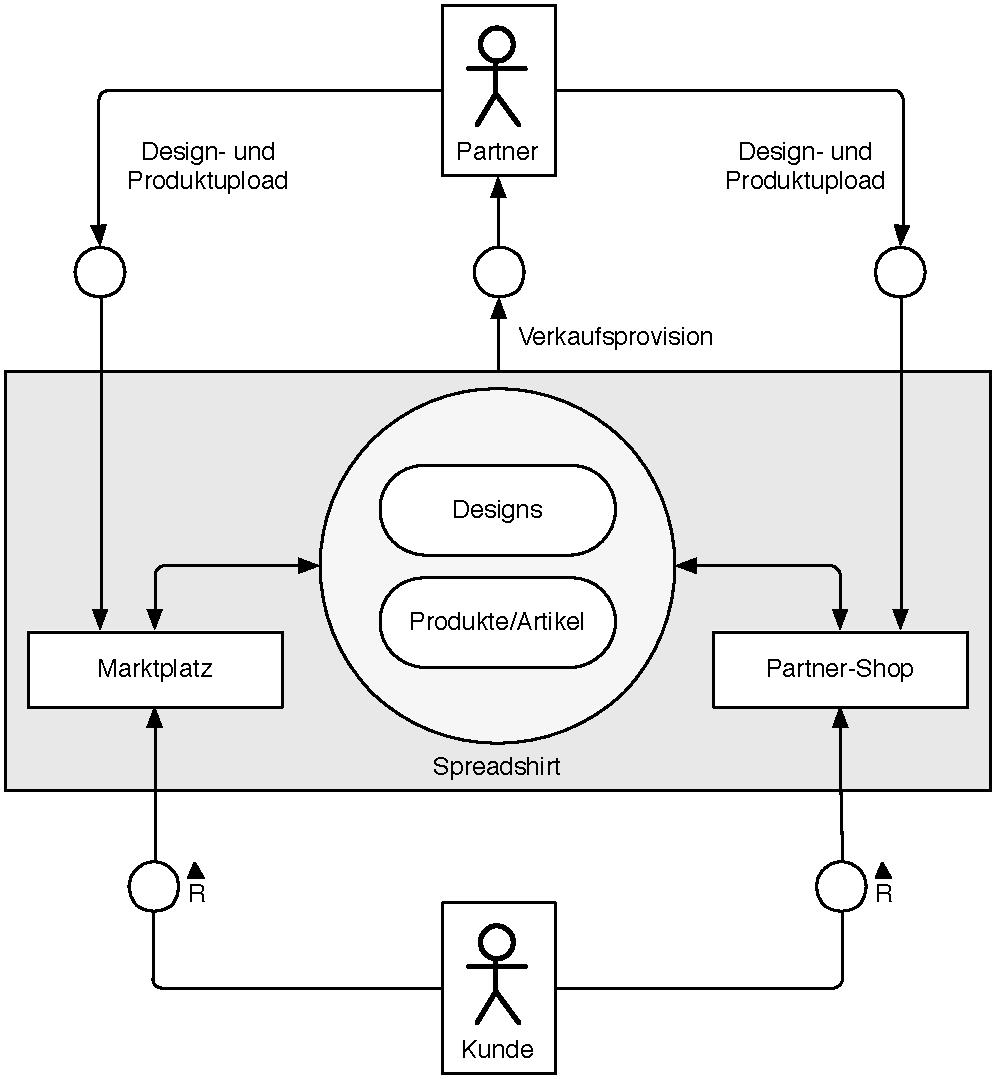
\includegraphics[width=0.7\textwidth]{how_spreadshirt_works}
\end{center}
\caption{Spreadshirt-Bereiche und Benutzer}
\end{figure}

Um also das Ziel zu erreichen, Themen und Assoziationen aus den Tags zu extrahieren, muss dieses spezifische Problem gelöst werden. Spam lässt sich nur schwer unterdrücken, so dass diesem bei der Auswertung der Daten besondere Aufmerksamkeit gewidmet werden muss.

Spreadshirt agiert international, so dass auf sprachliche und kulturelle Unterschiede Rücksicht genommen werden sollte. Viele Themen sind national unterschiedlich besetzt. Dies sollte in den Beziehungen der Tags untereinander widergespiegelt werden.

Der Datenbestand der Spreadshirt-Plattform in Europa besteht aus circa 2 Millionen Tags, 6 Millionen Designs, 14 Millionen Produkten, 6 Millionen registrierten Nutzern und \num{750000} eröffneten Partner-Shops.

\label{platforms}
Spreadshirt betreibt aus historischen gründen zwei Plattformen, deren Datenbestände größtenteils voneinander getrennt sind. Jeweils eine Plattform ist für den nordamerikanischen und den europäischen Markt zuständig. Im Kontext dieser Arbeit wird die europäische Plattform als Ausgangsbasis für alle Betrachtungen gewählt.

Der Nutzen dieser Arbeit für Spreadshirt besteht vor allem in der Verbesserung der Suche und des Durchstöberns des Marktplatzes. Den Kunden soll erleichtert werden, Designs zu ihren Wunschthemen zu finden, die ihren Vorstellungen entsprechen. Des Weiteren können diverse Marketingmaßnahmen von den Ergebnissen dieser Arbeit profitieren.

\section{Verwandte Arbeiten}

Die Herstellung von semantischen Beziehungen in Tag-Daten ist Gegenstand vieler Arbeiten. Diese beschäftigen sich meist mit Daten aus so genannten Folksonomies, also Sammlungen von Tags aus Systemen, bei denen alle Nutzer Inhalte verschlagworten können.

\textcite{bks2006} beschreiben einen auf Kookkurenz basierenden Ansatz, miteinander verwandte Tags zu Clustern zusammenzufassen. Dabei wird die Ähnlichkeit nicht nur durch die Menge, sondern auch durch die Verteilung der Häufigkeiten der gemeinsamen Vorkommen der Tags definiert. Dadurch ergeben sich bereits bei Berechnung des Ähnlichkeitsmaßes Cluster, die dann mit einem partitionierenden Algorithmus weiter geteilt werden.

In der Arbeit von \textcite{ps2006} wird ein Ansatz beschrieben, eine Ontologie aus den Daten der Foto-Plattform \emph{Flickr} herzustellen. Dazu wird versucht, ebenfalls auf Basis von Kookkurenzen, nicht nur Cluster von Tags, sondern hierarchische Beziehungen zwischen eben diesen zu ermitteln. Diese Beziehungen werden durch die Analyse der getaggten Inhalte hergestellt, indem ermittelt wird, welche der getaggten Inhalte Teilmengen voneinander sind.

\textcite{kss2010} arbeiten ebenfalls mit dem Ansatz, auf Basis eines Kookkurenzgraphen Cluster von Tags zu bilden. Die Kookkurenz wird mit den bekannten Maßen Dice, Jaccard und Cosinus berechnet. Als Clusteringalgorithmen kommen Single-Link, Complete-Link und Group-Average zum Einsatz. Die Arbeit legt besonderen Wert auf die Rolle der Cluster zur Verbesserung von Suchoberflächen. Daher werden auch Tests mit Benutzern durchgeführt und die Ergebnisse evaluiert.

\textcite{mcf2009} beschäftigen sich mit der Motivation und Erkennung von Spam in Tagging-Systemen. Es werden verschiedene Merkmale von Spam identifiziert und darauf basierend eine Klassifikation erstellt. Diese Merkmale konzentrieren sich vor allem auf Systeme, in denen es allen Benutzern erlaubt ist, Tags zu vergeben.

\section{Aufbau der Arbeit}